\documentclass{beamer}
\usetheme{CambridgeUS}
\usecolortheme{beaver}
\usepackage{xeCJK}
\usepackage{hyperref}

\usefonttheme[onlymath]{serif}
\begin{document} 

\begin{frame}
    \title{生生函数的运算与组合计数问题} 
    \begin{titlepage}
    \end{titlepage}
\end{frame} 

\section{生成函数} 

\begin{frame}{生成函数是啥}
    \begin{itemize}
        \item 想必大家已经很熟练了
        \item 对于数列$\{a_i\}$,我们定义它的普通生成函数(OGF)和指数生成函数(EGF)分别为
        $$\begin{aligned}
            A(x) &= \sum_{i\geq 0} a_i x^i\\
            \hat A(x) &= \sum_{i\geq 0} a_i \frac{x^i}{i!}
        \end{aligned}$$\pause
        \item 普通生成函数解决无标号问题,指数生成函数解决有标号问题
    \end{itemize}
\end{frame}

\begin{frame}{生成函数是啥}
    \begin{itemize}
        \item 两个普通生成函数的乘积$A(x)\times B(x)$可以理解为,从$A$中选择一个元素,再从$B$中选取一个元素,然后再将它们拼接起来\pause
        \item 比如说,有两个不相同的骰子,问有多少种方式使得两个骰子朝上的点数之和为8\pause
        \item 答案的生成函数为$(x + x^2 + x^3 + x^4 + x^5 + x^6)^2$
    \end{itemize}
\end{frame}

\begin{frame}{生成函数是啥}
    \begin{itemize}
        \item 两个指数生成函数的乘积$\hat A(x)\times \hat B(x)$可以理解为,$\hat A$中的元素内部已经分配好了编号,$\hat B$中的元素也已经分配好了编号。现在要将这两个序列中的元素组合起来,并且重新分配编号,且不能改变$\hat A,\hat B$中编号大小的相对顺序\pause
        $$\begin{aligned}
            \hat C(x) &= \hat A(x)\times \hat B(x)\\
            \frac{C_n}{n!} &= \sum_{i + j = n}\frac{A_i}{i!}\times \frac{B_j}{j!}\\
            C_n &= \sum_{i + j = n}A_i\times B_j\times {i + j\choose i}
        \end{aligned}$$
    \end{itemize}
\end{frame}

\begin{frame}{非常小的练习(我找不到题了)}
    \begin{itemize}
        \item 为了保证大家都在线,这里有两个简单的小练习
        \item 设$a_n$表示将$n$个完全相同的球放入编号为$1\sim 5$的篮子的方案数,其中编号为$1,2$的篮子中的球数必须是偶数,剩下的三个篮子每个篮子中的球数必须介于$3\sim 5$之间,求$a_n$的OGF
        \item 设$a_n$表示将$n$个不同的球放入$k$个不同的盒子的方案数,盒子可以是空的,求$a_n$的EGF
    \end{itemize}
\end{frame}

\begin{frame}{非常重要的展开式}
    \begin{itemize}
        \item 二项式定理
        \item $1 + x + x^2 + x^3 + \cdots = \frac{1}{1 - x}$
        \item $x + \frac{x^2}{2} + \frac{x^3}{3} + \cdots = -\ln(1 - x)$
        \item $1 + x + \frac{x^2}{2!} + \frac{x^3}{3!} + \cdots = \exp(x)$
    \end{itemize}
\end{frame}

\begin{frame}{多项式求逆}
    \begin{block}{问题}
        已知$A(x)\times B(x) \equiv 1\pmod {x^n}$,给出$A(x)$,求$B(x)$\newline
        保证$A_0\neq 0$
    \end{block} \pause
    \begin{itemize}
        \item 假设已经求出了$B'(x)$满足$A(x)\times B'(x)\equiv 1\pmod {x^{\lceil\frac n2\rceil}}$\pause
        $$\begin{aligned}
            A(x)\times B(x)&\equiv 1\pmod {x^{\lceil\frac n2\rceil}}\\ 
            \Rightarrow B(x)&\equiv B'(x) \pmod {x^{\lceil\frac n2\rceil}}\\ \pause
            B(x)^2 - 2B(x)B'(x) + B'(x)^2 &\equiv 0\pmod {x^n}\\ \pause
            B(x) - 2B'(x) + B'(x)^2A(x) &\equiv 0\pmod{x^n}\\
            2B'(x) - B'(x)^2A(x) &\equiv B(x)\pmod{x^n} 
        \end{aligned}$$
    \end{itemize}
\end{frame}

\begin{frame}{多项式$\ln$}
    \begin{block}{问题}
        已知$A(x)\equiv \ln B(x) \pmod {x^n}$,给出$B(x)$,求$A(x)$
    \end{block} \pause
    \begin{itemize}
        \item 相信大家都没有忘记小学三年级教的求导和积分 \pause
        $$\begin{aligned}
            A'(x) &= \frac{B'(x)}{B(x)}
        \end{aligned}$$ \pause
        \item 对$B(x)$求逆之后做一次NTT,再积分回去即可科技为了你
    \end{itemize}
\end{frame}

\begin{frame}{关于泰勒展开}
    \begin{itemize}
        \item 将多项式$F(x)$展开为无穷级数的形式 \pause
        \item 每一个$F(x)$,都有其唯一确定的导函数$F'(x)$ 
        \item 比如$F(x) = x^3 + 3$,我们可以得到$F'(x) = 3x^2$ \pause
        \item 但是我们不能逆用这个过程,因为有很多函数的导函数都是$F'(x) = 3x^2$,具体来说,这类函数是$F(x) = x^3 + C$ \pause
        \item 有一句话说得很好:原函数的信息=导函数的信息+初始值信息 \pause
    \end{itemize}
\end{frame}

\begin{frame}{关于泰勒展开}
    \begin{itemize}
        \item 我们选择一个点$x_0$来获取$F(x)$的初始值信息,我们将$x_0$称为展开点 \pause
        \item 接下来考虑$x_0 = 0$的情况 \pause
        $$\begin{aligned}
            F(x) &= \int_{0}^x F'(x) \,\mathrm{d}x + F(0)\\
            &= \int_{0}^x \left[\int_{0}^x F''(x) \,\mathrm{d}x + F'(0)\right] \,\mathrm{d}x + F(0)\\
            &= \int_{0}^x \int_{0}^x F''(x) \,\mathrm{d}x \,\mathrm{d}x + \int_{0}^x F'(0) \,\mathrm{d}x + F(0)
        \end{aligned}$$
    \end{itemize}
\end{frame}

\begin{frame}{多来几项}
    \begin{itemize}
        \item 可以发现最终$F(x)$被展开成了如下的形式 \pause
        $$\begin{aligned}
            F(x) &= F(0) + \int_{0}^x F'(0) \,\mathrm{d}x + \int_{0}^x \int_{0}^x F''(0) \,\mathrm{d}x\,\mathrm{d}x + \cdots\\
            &= F(0) + \frac{F'(0)x}{1} + \frac{F''(0)x^2}{1\times 2} + \cdots\\
            &= \sum_{i\geq 0} \frac{F^{(i)}(0)x^i}{i!}
        \end{aligned}$$
    \end{itemize}
\end{frame}

\begin{frame}{更一般的情况}
    \begin{itemize}
        \item 假如展开点不是$0$,而是$a$,该怎么办 \pause
        $$\begin{aligned}
            F(x) &= \int_{a}^x F'(x) \,\mathrm{d}x + F(a)\\
            &= F(a) + \int_{a}^x F'(a) \,\mathrm{d}x + \int_{a}^x \int_{a}^x F''(a) \,\mathrm{d}x \,\mathrm{d}x + \cdots
        \end{aligned}$$ \pause
        \item 令$u = x - a$,应用换元积分 \pause
        $$\begin{aligned}
            F(x) &= F(a) + \int_{0}^{u} F'(a) \,\mathrm{d}u + \int_{0}^{u} \int_{0}^{u} F''(a) \,\mathrm{d}u \,\mathrm{d}u + \cdots\\
            &= \sum_{i\geq 0} \frac{F^{(i)}(a)u^i}{i!} = \sum_{i\geq 0} \frac{F^{(i)}(a)(x - a)^i}{i!}
        \end{aligned}$$
    \end{itemize}
\end{frame}

\begin{frame}{牛顿迭代}
    \begin{block}{问题}
        已知$G[F(x)] \equiv 0\pmod {x^n}$,给出$G(x)$,求$F(x)$
    \end{block} \pause
    \begin{itemize}
        \item 记$F_t(x)$表示经过$t$次迭代之后的$F(x)$,满足
        $$\begin{aligned}
            G[F_t(x)] \equiv 0\pmod{x^{2^t}}
        \end{aligned}$$ \pause
        \item 考虑泰勒展开公式,对于函数$H(x)$,选择展开点$x_0$,那么有
        $$\begin{aligned}
            H(x) = \sum_{i\geq 0}\frac{H^{(i)}(x_0)}{i!}(x - x_0)^i
        \end{aligned}$$
    \end{itemize}
\end{frame}

\begin{frame}{牛顿迭代}
    \begin{itemize}
        \item 考虑将$G[F_{t+1}(x)]$从$F_t(x)$处展开 \pause
        $$\begin{aligned}
            G[F_{t+1}(x)]&=\sum_{i\geq 0}\frac{G^{(i)}[F_t(x)]}{i!}[F_{t+1}(x)-F_t(x)]^i\\ 
            &= G[F_t(x)] + G'[F_t(x)]\times [F_{t+1}(x) - F_t(x)] + \sum_{i\geq 2}\cdots\\  \pause
            0&\equiv G[F_t(x)] + G'[F_t(x)]\times [F_{t+1}(x) - F_t(x)]\pmod {x^{2^{t+1}}}\\ 
            F_{t+1}(x)&\equiv F_t(x) - \frac{G[F_t(x)]}{G'[F_t(x)]}\pmod {x^{2^{t + 1}}}
        \end{aligned}$$ \pause
        \item 注意这里的$G'[F_t(x)]$是先求出$G'(x)$,再代入$F_t(x)$,并非对$G[F_t(x)]$求导
    \end{itemize}
\end{frame}

\begin{frame}{多项式$\exp$}
    \begin{block}{问题}
        已知$A(x)\equiv \exp B(x) \pmod {x^n}$,给出$B(x)$,求$A(x)$
    \end{block} \pause
    \begin{itemize}
        \item 构造函数$G(x)$满足$G[A(x)] = 0$ \pause
        \item $G[A(x)] = \ln A(x) - B(x)$ \pause
        \item 应用牛顿迭代公式,可以得到 \pause
        $$\begin{aligned}
            G'[A(x)] &= \frac{1}{A(x)}\\
            F_{t+1}(x) &\equiv F_t(x) - \frac{G[F_t(x)]}{G'[F_t(x)]}\pmod {x^{2^{t + 1}}}\\
            &\equiv F_t(x)[1 - \ln F_t(x) + B(x)]\pmod {x^{2^{t + 1}}}
        \end{aligned}$$
    \end{itemize}
\end{frame}

\begin{frame}{来$k$道题}
    \begin{block}{经典问题}
        有若干种颜色不同的骨牌,其中大小为$1\times i$的骨牌共有$a_i$种,每种骨牌数量无限,问恰好填满$1\times n$的格子的方法。颜色相同的骨牌之间没有区别
        $$\begin{aligned}
            a_i, n\leq 10^5
        \end{aligned}$$
    \end{block}
\end{frame}

\begin{frame}{经典问题}
    \begin{itemize}
        \item 设$a$的OGF为$A(x)$,可以看出答案的OGF为
        $$\begin{aligned}
            \sum_{i\geq 0}A(x)^i=\frac{1}{1 - A(x)}
        \end{aligned}$$
        \item 非常良心
    \end{itemize}
\end{frame}

\begin{frame}{另一道经典问题}
    \begin{block}{论文中的题}
        给定集合$S$和正整数$n$,求有多少个$n$阶置换$p$,满足$p$分解之和每一个轮换的大小都在$S$内
        $$\begin{aligned}
            n\leq 10^5
        \end{aligned}$$
    \end{block}
\end{frame}

\begin{frame}{论文中的题}
    \begin{itemize}
        \item 置换与分解出的轮换一一对应\pause
        \item 假设原置换分解出的一个轮换长度为$n$,那么这个轮换中的元素一共有$(n-1)!$种排列方式\pause
        \item 原置换由若干个这样的轮换组成,且轮换与轮换之间是无序的\pause
        \item 写出一个轮换的EGF\pause
        $$\begin{aligned}
            \hat F(x) = \sum_{i\in S}(i-1)!\frac{x^i}{i!}
        \end{aligned}$$
    \end{itemize}
\end{frame}

\begin{frame}{论文中的题}
    \begin{itemize}
        \item 枚举最终的置换是由多少个轮换组成的,由于轮换是无序的,因此要除以一个阶乘\pause
        $$\begin{aligned}
            \hat G(x) = \sum_{i\geq 0}\frac{F(x)^i}{i!}
        \end{aligned}$$
        \item 喜闻乐见的$\exp$
    \end{itemize}
\end{frame}

\begin{frame}{经典问题}
    \begin{block}{论文中的题*2}
        你有若干种不同的物品,其中体积为$i$的物品有$a_i$种,每种物品有无限个。求选取物品恰好装满容量为$n$的背包的方案数
        $$n\leq 10^5$$
    \end{block}
\end{frame}

\begin{frame}{经典问题}
    \begin{itemize}
        \item 设$F(x)$是答案的OGF,$G(x)$是$\{a_i\}$的OGF \pause
        $$\begin{aligned}
            F(x)&=\prod_{i=1}^n(1+x^i+x^{2i}+x^{3i}+\cdots)^{a_i}\\
            &=\prod_{i=1}^n(\frac{1}{1-x^i})^{a_i}\\
            &=\exp\left(-\sum_{i=1}^na_i\ln(1-x^i)\right)\\
            &=\exp\left(\sum_{i=1}^na_i\sum_{j\geq 1}\frac{x^{ij}}{j}\right)\\
            &=\exp\left(\sum_{j\geq 1}\frac{G(x^j)}{j}\right)
        \end{aligned}$$
    \end{itemize}
\end{frame}

\begin{frame}{一道奇妙的题}
    \begin{block}{一道来自纪中的题}
        \begin{itemize}
            \item $n$个格子排成一行,你可以进行$m$次操作。\par
            \item 在第$i$次操作中,你可以选择两个下标$l,r(l\leq r)$,然后将第$l$个到第$r$个格子都染成颜色$i$,要求这$m$次操作之后所有格子都被染上了颜色\par
            \item 问最后可能出现的颜色序列一共有多少种
            $$\begin{aligned}
                n,m\leq 10^6
            \end{aligned}$$
        \end{itemize}
    \end{block}
\end{frame}

\begin{frame}{一道奇妙的题}
    \begin{itemize}
        \item 首先如何判断一个序列是否合法 \pause
        \item 最后一次加入的颜色必定在序列中出现。如果删去最后一次加入的颜色,那么倒数第二种颜色要么不出现,要么一定是连续的 \pause
        \item 设$dp[i][j]$表示考虑了前$i$种颜色,共有$j$个格子被染过色的方案数 \pause
        $$\begin{aligned}
            dp[i][j] = dp[i - 1][j] + \sum_{k = 0}^{j - 1}dp[i - 1][k]\times (k + 1)
        \end{aligned}$$
    \end{itemize}
\end{frame}

\begin{frame}{一道奇妙的题}
    \begin{itemize}
        \item 看起来非常不可优化 \pause
        \item 先把$\sum$前面的那个当前颜色不染色的情况拿掉,即假设在最终的序列中每种颜色都出现了,最后乘一个组合数即可 \pause
        $$\begin{aligned}
            dp[i][j] &= \sum_{k = 0}^{j - 1} dp[i - 1][k]\times (k + 1)\\
            &= \sum_{k = 0}^{j - 2} dp[i - 1][k]\times (k + 1) + dp[i - 1][j - 1]\times j\\
            &= dp[i][j - 1] + dp[i - 1][j - 1] \times j
        \end{aligned}$$
    \end{itemize}
\end{frame}

\begin{frame}{一道奇妙的题}
    \begin{itemize}
        \item 将$dp$看作是在$n\times m$的格子上走,这个网格有$n$行$m$列 \pause
        \item 注意这里行相当于$dp$的第二维,列相当于$dp$的第一维 \pause
        \item 那么相当于从$(0,0)$出发,每次可以往下走一格,方案数为$1$;或者往右下走一格,方案数为$j+1$ \pause
        \begin{center}
            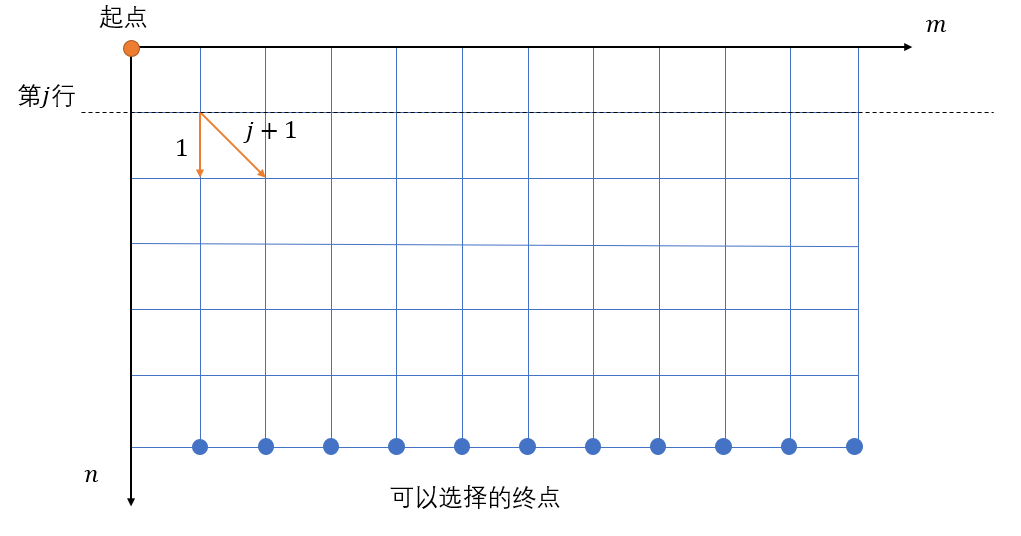
\includegraphics[scale = 0.25]{1.png}
        \end{center}
    \end{itemize}
\end{frame} 

\begin{frame}{一道奇妙的题}
    \begin{itemize}
        \item 我们需要分别求出,到达每个终点的所有路径的权值之和 \pause
        \item 可以发现每一步都必然会导致所在的行$+1$,因此我们考虑按行构造生成函数 \pause
        \item 我们用$x$的指数来代表当前所在的列数,每次我们要么使得当前的列不变,要么使得当前的列$+1$ \pause
        \item 因此$F_i=dp[i][n]$的OGF为
        $$\begin{aligned}
            F(x) = x\prod_{i = 1} ^ {n - 1}(1 + (i + 1)x)
        \end{aligned}$$ 
        \item 注意第一步必定是由$(0,0)$走到$(1,1)$,因此这里要乘上$x$
    \end{itemize}
\end{frame}

\begin{frame}{一道奇妙的题}
    \begin{itemize}
        \item 很不幸,这个东西仍然不好求 \pause
        \item 再将这个多项式转化一下 \pause
        \item 由于总步数为$n$,因此如果我们知道了向下走了多少步,那么我们也就知道了向右下走了多少步 \pause
        \item 将向下走一步看作$x$,那么最终多项式中$x^i$的系数就是原多项式中$x^{n - i}$的系数 \pause
        $$\begin{aligned}
            F_1(x) = \prod_{i = 1}^{n - 1} (x + i + 1)
        \end{aligned}$$
    \end{itemize}
\end{frame}

\begin{frame}{这种奇形怪状的东西是可以求的}
    \begin{itemize}
        \item 记$G_t(x)=\prod_{i = 1} ^ {2 ^ t} (x + i + 1)$ \pause
        \item 如果我们能算出所有的$G$,那么我们就可以用类似快速幂的方法算出原多项式 \pause
        $$\begin{aligned}
            G_{t + 1}(x) = G_t(x)\times G_t(x + 2^t)
        \end{aligned}$$ \pause
        \item 记$a_i = [x^i]G_t(x),b = 2^t$ \pause
        $$\begin{aligned}
            G_{t}(x + b) = \sum_{i\geq 0}a_i\times (x + b)^i
        \end{aligned}$$ \pause
        \item 二项式定理展开
    \end{itemize}
\end{frame}

\begin{frame}{这一页是展开}
    $$\begin{aligned}
        G_t(x + b) &= \sum_{i\geq 0}a_i\times (x + b)^i\\
        &= \sum_{i\geq 0}a_i\sum_{j = 0}^i{i\choose j}x^jb^{i-j}\\
        &= \sum_{j\geq 0}x^j\sum_{i\geq j}a_ib^{i-j}\frac{i!}{j!(i-j)!}\\
        &= \sum_{j\geq 0}\frac{x^j}{j!}\sum_{i\geq j}(a_ii!)\times \frac{b^{i - j}}{(i - j)!}
    \end{aligned}$$ \pause
    \begin{itemize}
        \item 记$A(x) = \sum_{i\geq 0}a_{i}i!x^{n-i},B(x)=\sum_{i\geq 0}\frac{b^i}{i!}x^i$
        \item 第$j$项的$\sum$为$A(x)\times B(x)$的第$n-j$项的系数
    \end{itemize}
\end{frame}

\end{document}